\documentclass{standalone}
\usepackage{tikz}
\usetikzlibrary{patterns, positioning}

\begin{document}
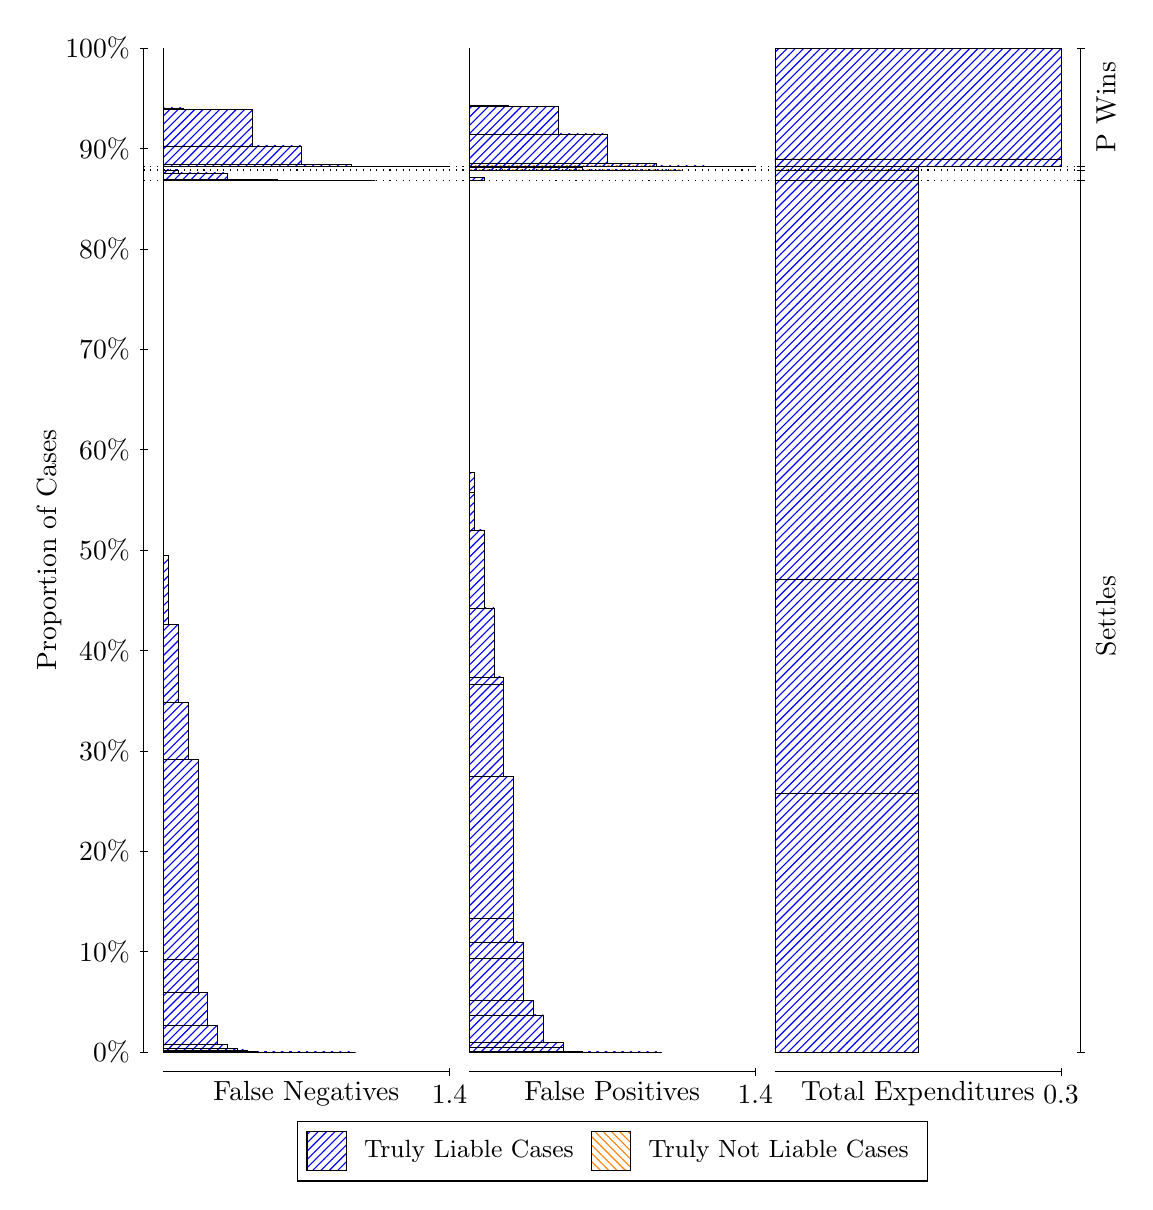
\begin{tikzpicture}
\draw[black, very thin] (1.5,1.75) -- (1.5,14.5);
\node[rotate=90, anchor=center] at (0.3, 8.125) {Proportion of Cases};
\draw[black, very thin] (1.45,1.75) -- (1.55,1.75);
\node[anchor=east] at (1.45, 1.75) {0\%};
\draw[black, very thin] (1.45,3.025) -- (1.55,3.025);
\node[anchor=east] at (1.45, 3.025) {10\%};
\draw[black, very thin] (1.45,4.3) -- (1.55,4.3);
\node[anchor=east] at (1.45, 4.3) {20\%};
\draw[black, very thin] (1.45,5.575) -- (1.55,5.575);
\node[anchor=east] at (1.45, 5.575) {30\%};
\draw[black, very thin] (1.45,6.85) -- (1.55,6.85);
\node[anchor=east] at (1.45, 6.85) {40\%};
\draw[black, very thin] (1.45,8.125) -- (1.55,8.125);
\node[anchor=east] at (1.45, 8.125) {50\%};
\draw[black, very thin] (1.45,9.4) -- (1.55,9.4);
\node[anchor=east] at (1.45, 9.4) {60\%};
\draw[black, very thin] (1.45,10.675) -- (1.55,10.675);
\node[anchor=east] at (1.45, 10.675) {70\%};
\draw[black, very thin] (1.45,11.95) -- (1.55,11.95);
\node[anchor=east] at (1.45, 11.95) {80\%};
\draw[black, very thin] (1.45,13.225) -- (1.55,13.225);
\node[anchor=east] at (1.45, 13.225) {90\%};
\draw[black, very thin] (1.45,14.5) -- (1.55,14.5);
\node[anchor=east] at (1.45, 14.5) {100\%};

\draw[black, very thin] (13.4,1.75) -- (13.4,14.5);
\draw[black, very thin] (13.35,1.75) -- (13.45,1.75);
\node[anchor=west] at (13.35, 1.75) {};
\draw[black, very thin] (13.35,12.822) -- (13.45,12.822);
\node[anchor=west] at (13.35, 12.822) {};
\draw[black, very thin] (13.35,12.951) -- (13.45,12.951);
\node[anchor=west] at (13.35, 12.951) {};
\draw[black, very thin] (13.35,13.001) -- (13.45,13.001);
\node[anchor=west] at (13.35, 13.001) {};
\draw[black, very thin] (13.35,14.5) -- (13.45,14.5);
\node[anchor=west] at (13.35, 14.5) {};

\draw[black, very thin, pattern color=blue, pattern=north east lines] (1.75,1.75) rectangle (4.1931,1.75);
\draw[black, very thin, pattern color=blue, pattern=north east lines] (1.75,1.75) rectangle (3.9425,1.75);
\draw[black, very thin, pattern color=blue, pattern=north east lines] (1.75,1.75) rectangle (3.692,1.75);
\draw[black, very thin, pattern color=blue, pattern=north east lines] (1.75,1.75) rectangle (3.5667,1.75);
\draw[black, very thin, pattern color=blue, pattern=north east lines] (1.75,1.75) rectangle (3.4414,1.75);
\draw[black, very thin, pattern color=blue, pattern=north east lines] (1.75,1.75) rectangle (3.3161,1.75);
\draw[black, very thin, pattern color=blue, pattern=north east lines] (1.75,1.75) rectangle (3.1908,1.75);
\draw[black, very thin, pattern color=blue, pattern=north east lines] (1.75,1.75) rectangle (3.0655,1.7507);
\draw[black, very thin, pattern color=blue, pattern=north east lines] (1.75,1.7507) rectangle (2.9402,1.7597);
\draw[black, very thin, pattern color=blue, pattern=north east lines] (1.75,1.7597) rectangle (2.8149,1.7597);
\draw[black, very thin, pattern color=blue, pattern=north east lines] (1.75,1.7597) rectangle (2.8149,1.7763);
\draw[black, very thin, pattern color=blue, pattern=north east lines] (1.75,1.7763) rectangle (2.6897,1.8004);
\draw[black, very thin, pattern color=blue, pattern=north east lines] (1.75,1.8004) rectangle (2.5644,1.8474);
\draw[black, very thin, pattern color=blue, pattern=north east lines] (1.75,1.8474) rectangle (2.4391,2.0898);
\draw[black, very thin, pattern color=blue, pattern=north east lines] (1.75,2.0898) rectangle (2.4391,2.0898);
\draw[black, very thin, pattern color=blue, pattern=north east lines] (1.75,2.0898) rectangle (2.3138,2.5074);
\draw[black, very thin, pattern color=blue, pattern=north east lines] (1.75,2.5074) rectangle (2.1885,2.5085);
\draw[black, very thin, pattern color=blue, pattern=north east lines] (1.75,2.5085) rectangle (2.1885,2.9223);
\draw[black, very thin, pattern color=blue, pattern=north east lines] (1.75,2.9223) rectangle (2.1885,5.4641);
\draw[black, very thin, pattern color=blue, pattern=north east lines] (1.75,5.4641) rectangle (2.0632,6.1923);
\draw[black, very thin, pattern color=blue, pattern=north east lines] (1.75,6.1923) rectangle (1.9379,7.1829);
\draw[black, very thin, pattern color=blue, pattern=north east lines] (1.75,7.1829) rectangle (1.8126,8.0581);
\draw[black, very thin, pattern color=blue, pattern=north east lines] (1.75,8.0581) rectangle (1.8126,8.0581);
\draw[black, very thin, pattern color=orange, pattern=north west lines] (1.75,8.0581) rectangle (1.75,8.0581);
\draw[black, very thin, pattern color=blue, pattern=north east lines] (1.75,8.0581) rectangle (1.75,12.822);
\draw[black, very thin, pattern color=blue, pattern=north east lines] (1.75,12.822) rectangle (4.4437,12.822);
\draw[black, very thin, pattern color=blue, pattern=north east lines] (1.75,12.822) rectangle (3.8172,12.822);
\draw[black, very thin, pattern color=blue, pattern=north east lines] (1.75,12.822) rectangle (3.1908,12.829);
\draw[black, very thin, pattern color=blue, pattern=north east lines] (1.75,12.829) rectangle (2.5644,12.913);
\draw[black, very thin, pattern color=blue, pattern=north east lines] (1.75,12.913) rectangle (1.9379,12.951);
\draw[black, very thin, pattern color=orange, pattern=north west lines] (1.75,12.951) rectangle (1.75,12.951);
\draw[black, very thin, pattern color=blue, pattern=north east lines] (1.75,12.951) rectangle (1.9379,12.951);
\draw[black, very thin, pattern color=orange, pattern=north west lines] (1.75,12.951) rectangle (1.75,12.951);
\draw[black, very thin, pattern color=blue, pattern=north east lines] (1.75,12.951) rectangle (1.75,13.001);
\draw[black, very thin, pattern color=blue, pattern=north east lines] (1.75,13.001) rectangle (5.3833,13.001);
\draw[black, very thin, pattern color=blue, pattern=north east lines] (1.75,13.001) rectangle (4.7569,13.001);
\draw[black, very thin, pattern color=blue, pattern=north east lines] (1.75,13.001) rectangle (4.1305,13.019);
\draw[black, very thin, pattern color=blue, pattern=north east lines] (1.75,13.019) rectangle (3.504,13.258);
\draw[black, very thin, pattern color=blue, pattern=north east lines] (1.75,13.258) rectangle (3.2534,13.258);
\draw[black, very thin, pattern color=blue, pattern=north east lines] (1.75,13.258) rectangle (2.8776,13.725);
\draw[black, very thin, pattern color=blue, pattern=north east lines] (1.75,13.725) rectangle (2.627,13.725);
\draw[black, very thin, pattern color=blue, pattern=north east lines] (1.75,13.725) rectangle (2.2511,13.725);
\draw[black, very thin, pattern color=blue, pattern=north east lines] (1.75,13.725) rectangle (2.0006,13.74);
\draw[black, very thin, pattern color=orange, pattern=north west lines] (1.75,13.74) rectangle (1.75,13.74);
\draw[black, very thin, pattern color=blue, pattern=north east lines] (1.75,13.74) rectangle (1.75,14.5);
\draw[black, very thin, pattern color=orange, pattern=north west lines] (5.6333,1.75) rectangle (8.0764,1.75);
\draw[black, very thin, pattern color=blue, pattern=north east lines] (5.6333,1.75) rectangle (8.0764,1.75);
\draw[black, very thin, pattern color=orange, pattern=north west lines] (5.6333,1.75) rectangle (7.8259,1.75);
\draw[black, very thin, pattern color=blue, pattern=north east lines] (5.6333,1.75) rectangle (7.8259,1.75);
\draw[black, very thin, pattern color=orange, pattern=north west lines] (5.6333,1.75) rectangle (7.5753,1.75);
\draw[black, very thin, pattern color=blue, pattern=north east lines] (5.6333,1.75) rectangle (7.5753,1.75);
\draw[black, very thin, pattern color=blue, pattern=north east lines] (5.6333,1.75) rectangle (7.45,1.75);
\draw[black, very thin, pattern color=orange, pattern=north west lines] (5.6333,1.75) rectangle (7.3247,1.75);
\draw[black, very thin, pattern color=blue, pattern=north east lines] (5.6333,1.75) rectangle (7.3247,1.75);
\draw[black, very thin, pattern color=blue, pattern=north east lines] (5.6333,1.75) rectangle (7.1994,1.7501);
\draw[black, very thin, pattern color=orange, pattern=north west lines] (5.6333,1.7501) rectangle (7.0741,1.7501);
\draw[black, very thin, pattern color=blue, pattern=north east lines] (5.6333,1.7501) rectangle (7.0741,1.7527);
\draw[black, very thin, pattern color=blue, pattern=north east lines] (5.6333,1.7527) rectangle (6.9489,1.7536);
\draw[black, very thin, pattern color=orange, pattern=north west lines] (5.6333,1.7536) rectangle (6.8236,1.7536);
\draw[black, very thin, pattern color=blue, pattern=north east lines] (5.6333,1.7536) rectangle (6.8236,1.8083);
\draw[black, very thin, pattern color=orange, pattern=north west lines] (5.6333,1.8083) rectangle (6.8236,1.8083);
\draw[black, very thin, pattern color=blue, pattern=north east lines] (5.6333,1.8083) rectangle (6.8236,1.8745);
\draw[black, very thin, pattern color=blue, pattern=north east lines] (5.6333,1.8745) rectangle (6.6983,1.8764);
\draw[black, very thin, pattern color=orange, pattern=north west lines] (5.6333,1.8764) rectangle (6.573,1.8764);
\draw[black, very thin, pattern color=blue, pattern=north east lines] (5.6333,1.8764) rectangle (6.573,2.2206);
\draw[black, very thin, pattern color=blue, pattern=north east lines] (5.6333,2.2206) rectangle (6.4477,2.4033);
\draw[black, very thin, pattern color=orange, pattern=north west lines] (5.6333,2.4033) rectangle (6.3224,2.4033);
\draw[black, very thin, pattern color=blue, pattern=north east lines] (5.6333,2.4033) rectangle (6.3224,2.9373);
\draw[black, very thin, pattern color=blue, pattern=north east lines] (5.6333,2.9373) rectangle (6.3224,3.1486);
\draw[black, very thin, pattern color=blue, pattern=north east lines] (5.6333,3.1486) rectangle (6.1971,3.4439);
\draw[black, very thin, pattern color=blue, pattern=north east lines] (5.6333,3.4439) rectangle (6.1971,5.2514);
\draw[black, very thin, pattern color=orange, pattern=north west lines] (5.6333,5.2514) rectangle (6.0718,5.2514);
\draw[black, very thin, pattern color=blue, pattern=north east lines] (5.6333,5.2514) rectangle (6.0718,6.4164);
\draw[black, very thin, pattern color=blue, pattern=north east lines] (5.6333,6.4164) rectangle (6.0718,6.5143);
\draw[black, very thin, pattern color=blue, pattern=north east lines] (5.6333,6.5143) rectangle (5.9466,7.3896);
\draw[black, very thin, pattern color=blue, pattern=north east lines] (5.6333,7.3896) rectangle (5.8213,8.3801);
\draw[black, very thin, pattern color=blue, pattern=north east lines] (5.6333,8.3801) rectangle (5.696,8.8604);
\draw[black, very thin, pattern color=blue, pattern=north east lines] (5.6333,8.8604) rectangle (5.696,9.1083);
\draw[black, very thin, pattern color=blue, pattern=north east lines] (5.6333,9.1083) rectangle (5.6333,12.822);
\draw[black, very thin, pattern color=orange, pattern=north west lines] (5.6333,12.822) rectangle (5.8213,12.822);
\draw[black, very thin, pattern color=blue, pattern=north east lines] (5.6333,12.822) rectangle (5.8213,12.86);
\draw[black, very thin, pattern color=blue, pattern=north east lines] (5.6333,12.86) rectangle (5.6333,12.951);
\draw[black, very thin, pattern color=orange, pattern=north west lines] (5.6333,12.951) rectangle (8.327,12.951);
\draw[black, very thin, pattern color=blue, pattern=north east lines] (5.6333,12.951) rectangle (8.327,12.951);
\draw[black, very thin, pattern color=blue, pattern=north east lines] (5.6333,12.951) rectangle (7.7006,12.953);
\draw[black, very thin, pattern color=blue, pattern=north east lines] (5.6333,12.953) rectangle (7.0741,12.987);
\draw[black, very thin, pattern color=blue, pattern=north east lines] (5.6333,12.987) rectangle (6.4477,13.001);
\draw[black, very thin, pattern color=blue, pattern=north east lines] (5.6333,13.001) rectangle (5.8213,13.001);
\draw[black, very thin, pattern color=orange, pattern=north west lines] (5.6333,13.001) rectangle (9.2667,13.001);
\draw[black, very thin, pattern color=blue, pattern=north east lines] (5.6333,13.001) rectangle (9.2667,13.001);
\draw[black, very thin, pattern color=orange, pattern=north west lines] (5.6333,13.001) rectangle (8.6402,13.001);
\draw[black, very thin, pattern color=blue, pattern=north east lines] (5.6333,13.001) rectangle (8.6402,13.002);
\draw[black, very thin, pattern color=orange, pattern=north west lines] (5.6333,13.002) rectangle (8.0138,13.002);
\draw[black, very thin, pattern color=blue, pattern=north east lines] (5.6333,13.002) rectangle (8.0138,13.031);
\draw[black, very thin, pattern color=orange, pattern=north west lines] (5.6333,13.031) rectangle (7.3874,13.031);
\draw[black, very thin, pattern color=blue, pattern=north east lines] (5.6333,13.031) rectangle (7.3874,13.409);
\draw[black, very thin, pattern color=blue, pattern=north east lines] (5.6333,13.409) rectangle (6.7609,13.761);
\draw[black, very thin, pattern color=orange, pattern=north west lines] (5.6333,13.761) rectangle (6.5103,13.761);
\draw[black, very thin, pattern color=blue, pattern=north east lines] (5.6333,13.761) rectangle (6.5103,13.761);
\draw[black, very thin, pattern color=blue, pattern=north east lines] (5.6333,13.761) rectangle (6.1345,13.776);
\draw[black, very thin, pattern color=orange, pattern=north west lines] (5.6333,13.776) rectangle (5.8839,13.776);
\draw[black, very thin, pattern color=blue, pattern=north east lines] (5.6333,13.776) rectangle (5.8839,13.776);
\draw[black, very thin, pattern color=blue, pattern=north east lines] (5.6333,13.776) rectangle (5.8839,13.776);
\draw[black, very thin, pattern color=orange, pattern=north west lines] (5.6333,13.776) rectangle (5.6333,13.776);
\draw[black, very thin, pattern color=blue, pattern=north east lines] (5.6333,13.776) rectangle (5.6333,14.5);
\draw[black, very thin, pattern color=orange, pattern=north west lines] (9.5167,1.75) rectangle (11.333,1.75);
\draw[black, very thin, pattern color=blue, pattern=north east lines] (9.5167,1.75) rectangle (11.333,5.0307);
\draw[black, very thin, pattern color=orange, pattern=north west lines] (9.5167,5.0307) rectangle (11.333,5.0307);
\draw[black, very thin, pattern color=blue, pattern=north east lines] (9.5167,5.0307) rectangle (11.333,7.7524);
\draw[black, very thin, pattern color=orange, pattern=north west lines] (9.5167,7.7524) rectangle (11.333,7.7524);
\draw[black, very thin, pattern color=blue, pattern=north east lines] (9.5167,7.7524) rectangle (11.333,12.822);
\draw[black, very thin, pattern color=orange, pattern=north west lines] (9.5167,12.822) rectangle (11.333,12.822);
\draw[black, very thin, pattern color=blue, pattern=north east lines] (9.5167,12.822) rectangle (11.333,12.951);
\draw[black, very thin, pattern color=orange, pattern=north west lines] (9.5167,12.951) rectangle (11.333,12.951);
\draw[black, very thin, pattern color=blue, pattern=north east lines] (9.5167,12.951) rectangle (11.333,13.001);
\draw[black, very thin, pattern color=orange, pattern=north west lines] (9.5167,13.001) rectangle (13.15,13.001);
\draw[black, very thin, pattern color=blue, pattern=north east lines] (9.5167,13.001) rectangle (13.15,13.091);
\draw[black, very thin, pattern color=orange, pattern=north west lines] (9.5167,13.091) rectangle (13.15,13.091);
\draw[black, very thin, pattern color=blue, pattern=north east lines] (9.5167,13.091) rectangle (13.15,14.5);
\draw[black, dotted] (1.5,12.822) -- (13.4,12.822);
\draw[black, dotted] (1.5,12.951) -- (13.4,12.951);
\draw[black, dotted] (1.5,13.001) -- (13.4,13.001);
\draw[black, very thin] (1.75,1.5) -- (5.3833,1.5);
\node[anchor=north] at (3.5667, 1.5) {False Negatives};
\draw[black, very thin] (5.3833,1.45) -- (5.3833,1.55);
\node[anchor=north] at (5.3833, 1.45) {1.4};

\draw[black, very thin] (5.6333,1.5) -- (9.2667,1.5);
\node[anchor=north] at (7.45, 1.5) {False Positives};
\draw[black, very thin] (9.2667,1.45) -- (9.2667,1.55);
\node[anchor=north] at (9.2667, 1.45) {1.4};

\draw[black, very thin] (9.5167,1.5) -- (13.15,1.5);
\node[anchor=north] at (11.333, 1.5) {Total Expenditures};
\draw[black, very thin] (13.15,1.45) -- (13.15,1.55);
\node[anchor=north] at (13.15, 1.45) {0.3};

\node[black, centered, rotate=90] at (13.72, 7.2862) {Settles};


\node[black, centered, rotate=90] at (13.72, 13.751) {P Wins};

\draw (7.449999999999999,1.5) node[draw=none] (baseCoordinate) {};
\begin{scope}[align=center]
        \matrix[scale=0.5, draw=black, below=0.5cm of baseCoordinate, nodes={draw}, column sep=0.1cm]{
            \node[rectangle, draw, minimum width=0.5cm, minimum height=0.5cm, pattern=north east lines, pattern color=blue] {}; &
            \node[draw=none, font=\small] (B) {Truly Liable Cases}; &
            \node[rectangle, draw, minimum width=0.5cm, minimum height=0.5cm, pattern=north west lines, pattern color=orange] {}; &
            \node[draw=none, font=\small] (B) {Truly Not Liable Cases}; \\
            };
\end{scope}

\end{tikzpicture}
\end{document}